%\documentclass[letterpaper,12pt]{book}
%\usepackage[spanish]{babel}
%\usepackage{graphicx, color}
%\usepackage{amsmath}
%\usepackage{amscd}
%\usepackage{titlesec}
%\usepackage[latin1]{inputenc}
%\usepackage{listings}
%\usepackage{multicol}
%\usepackage{enumerate}
%\usepackage{amssymb}
%\usepackage{amsthm}
%\usepackage{syntonly}
%\usepackage{fancyhdr}
%\usepackage{verbatim}
%\usepackage{fancyvrb}
%\usepackage{hyperref}
%
%\begin{document}

%%%++++++++++++++++++++++++++++++++++++

Claramente los experimentos de frotación pueden electrificar un cuerpo, lo cual se ve claramente en la atracción de pedasitos de papel cuando le arrimamos una barra de vidrio o de plástico que frotamos previamente. El fenómeno de electrificción también puede verse en las chispas que salen cuando nos quitamos una camisa en ciertos lugares relativamente secos.

\section{Carga eléctrica}
Experimentalemente \textbf{Benjamin Franklin (1706-1790)} fue quien determinó que existen dos tipos de cargas eléctricas a las que llamó positivas y negativas. Él determinó que dos barras de vidrio o dos barras de hule (caucho) cargadas por frotación se repelen y dos barras, una de vidrio y otra de hule cargadas, se atraen. El experimento es exquematizado brevemente en la Figura... 

Posterior a esto se estableció una visión más moderna y concreta de la interacción eléctrica. Existen dos tipos de carga, una positiva (vidrio) y una negativa (hule), las cuales exiben una de las características fundamentales de la interacción eléctrica; ``\textbf{cargas de un mismo signo se repelen y cargas de signo contrario se atraen}", Figura ...

\subsection{Cuantización y conservación de la carga eléctrica}

En 1909 \textbf{Robert Millikan (1868-1953)} (CITAR EXPERIMENTO) encontró que las cargas eléctricas siempre se presentan en múltiplos enteros de una cantidad básica $e=1.609 \times 10^{-19}$ C, donde C es la unidad tomada para la carga eléctrica en el sistema internacional SI. Dado, lo anterior, un cuerpo cargado eléctricamente tiene una carga neta $q$, tal que:

\begin{equation}
q=\pm N e \hspace{0.2 cm},\hspace{0.2 cm} N \in Z
\end{equation}

Los cuerpos cargados tienen una carga neta $+Ne$ y los cuerpos electricamente negativos tienen una carga neta $-Ne$. Por ejemplo, la carga eléctrica del electrón es $-e$ y la carga eléctrica del protón es $+e$. 
\subsection{Ley de Coulomb}

\textbf{Charles Coulomb (1736-1806)} midió la magnitud de la fuerza eléctrica entre dos objetos cagados que había sido estudiada y no cuantificada por Benjamin Franklin. Coulomb usó una balanza de tosión y determinó que la fuerza de atacción o repulsión eléctrica entre dos cargas $q_1$ y $q_2$ separadas una distancia $r$ está dada por:


\begin{equation}
F_e=k_e \dfrac{|q_1||q_2|}{r^2}=\dfrac{1}{4\pi \epsilon_0 } \dfrac{|q_1||q_2|}{r^2} ,
\end{equation}

donde $k_e=8.9875 \times 10^9$ Nm$^2$/C$^2$ y $\epsilon_0=8.8542 \times 10^12 $ C$^2$/N$^2$m$^2$ son constantes. La primera es llamada la constante eléctrica y la segunda es llamada la permitividad del 
espacio libre (vacío).

\begin{figure}[h]
\begin{center}
\includegraphics[scale=0.9]{electrostatica/coulomb}
\end{center}
\caption{Atracción y repulsión eléctrica entre cargas eléctricas}
\end{figure}

El caracter vectorial de dicha fuerza depende del signo de ambas cargas, ``\textbf{cargas de un mismo signo se repelen y cargas de signo contrario se atraen}".

\vspace{1.0 cm}

\textbf{EJEMPLO:} 

\begin{figure}[h]
\begin{center}
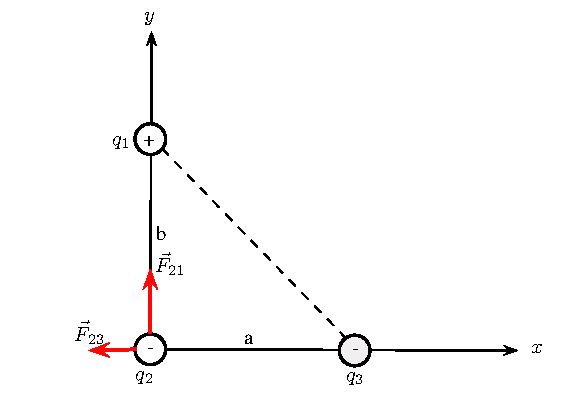
\includegraphics[scale=1.0]{electrostatica/interaccionelectrica1}
\end{center}
\caption{Fuerza neta sobre $q_2$}
\end{figure}

\begin{enumerate}
\item Calculemos la fuerza $\vec{F}_2$ que actua sobe la carga $q_2$ debido a las cargas $q_1$ y $q_3$. Use las cantidades dadas en la figura.

\begin{eqnarray}
\vec{F}_2=\vec{F}_{23}+\vec{F}_{21} =- k_e \dfrac{|q_2||q_3|}{a^2}\hat{i}+k_e \dfrac{|q_2||q_1|}{b^2}\hat{j}=k_e|q_2|\bigg[- \dfrac{|q_3|}{a^2}\hat{i}+\dfrac{q_1}{b^2}\hat{j}\bigg]
\end{eqnarray}

\item Calculemos el valor de la fuerza si $q_1=4 \mu$ C, $q_2=-2 \mu$ C, $q_3=-3\mu$ C, $a=15$ cm y $b= 10$ cm.
\begin{eqnarray}
\vec{F}_2=(-2.4 N \hat{i}+7.2 N \hat{j})
\end{eqnarray}
\item Ejercicio: Calcule la fuerza neta $\vec{F}_1$ y $\vec{F}_3$ que actúan sobre las cargas $q_1$ y $q_3$ respectivamente. Mueste que $\sum_{i=1}^{3} \vec{F}_i=\vec{F}_1+\vec{F}_2+\vec{F}_3=\vec{0}$.
\end{enumerate}

\textbf{EJEMPLO:} Dos masas puntuales $m$ muy pequeñas e iguales, forman dos péndulos de longitud $l$ (desprecie la masa de la cuerda). Debido a su repulsión mutua, las cuerdas forman un ángulo $\theta$ con la vertical, tal como se muestra en la figura. Calculemos la magnitud de la cada una de las cargas.

\vspace{0.4 cm}

\begin{figure}
\begin{center}
\includegraphics[scale=0.7]{electrostatica/interaccionelectrica2}
\end{center}
\caption{Rupulsión eléctrica entre pendulos de cargas y masas iguales}
\end{figure}

Según el diagrama de cuerpo mostrado en la figura:
\begin{eqnarray}
\rightarrow^{+} \sum_{i}F_{xi}=0 \Rightarrow F_e=T\sin\theta
\end{eqnarray}
\begin{eqnarray}
\uparrow^{+} \sum_{i}F_{yi}=0 \Rightarrow mg=T\cos\theta ,
\end{eqnarray}
además, la fuerza eléctrica $F_e$ está dada por:
\begin{eqnarray}
F_e=k_e \dfrac{q^2}{(2x)^2} 
\end{eqnarray}

Usando las ecuaciones anteriores y $\sin\theta=x/l$, se concluye que:
\begin{eqnarray}
|q|=\sqrt{\dfrac{4mg l^2}{k_e\cos\theta\sin^3\theta} } =(2l\sin\theta)\sqrt{4\pi \epsilon_0 mg \tan\theta }.
\end{eqnarray}

\section{Campo eléctrico}

\begin{figure}[h]
\begin{center}
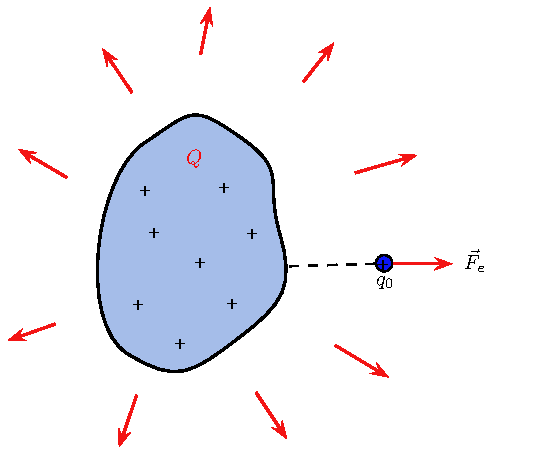
\includegraphics[scale=0.6]{electrostatica/campoelectrico1}
\end{center}
\caption{Definición de campo eléctrico}
\label{campoelectrico}
\end{figure}

El campo eléctrico $\vec{E}$ en un punto del espacio se define como la fuerza eléctrica $\vec{F}_e$ que actua sobre una carga de prueba ``positiva $q_0$'' colocada en dicho punto, dividida entre la carga de prueba.

\begin{equation}
%\boxed{
\vec{E}=\dfrac{\vec{F}_e}{q_0}
\end{equation}


\textit{Se dice que existe un campo eléctrico en la región del espacio que rodea al cuerpo de carga $Q$. Cuando otro cuerpo cargado entra a este campo eléctrico, una fuerza eléctrica actua sobre él.}

Note que el campo es producido por la carga $Q$ y no por la carga de prueba $q_0$. Además, la fuerza que actúa a la distacia (no es necesario tener un contacto físico entre las cargas) es la que nos permite definir el concepto de campo eléctrico. 
Por último, las dimensiones del campo eléctrico en el sistema internacional SI, serán N/C.

\vspace{0.5cm}

\textbf{Dirección del campo eléctrico $\rightarrow$ Líneas de campo}

\vspace{0.5cm}

La dirección establecida para el campo eléctrico es un convención, es debida al hecho de que la carga de prueba $q_0$ es tomada positiva. Si la carga $Q$ generadora del campo es positiva, entonces la línea de  acción de la fuerza diverge de la carga $Q$ y diremos que el campo eléctrico sale de las cargas positivas. Ahora, si $Q$ es negativa, entonces la linea de acción de la fuerza va hacia la carga $Q$ y diremos que el campo eléctrico entra a las cargas negativas (ver Figura \ref{direcciondelE}).

\begin{figure}[h]
\begin{center}
\includegraphics[scale=0.8]{electrostatica/direcciondelcampoelectrico}
\end{center}
\caption{Dirección del campo eléctrico. Líneas de campo}
\label{direcciondelE}
\end{figure}

Para el caso de una carga puntual (Figura \ref{direcciondelE}) el campo eléctrico es:

\begin{equation}
\vec{E}=k_e \dfrac{q}{r^2} \hat{u}_r= \dfrac{1}{4\pi \epsilon_0} \dfrac{q}{r^2} \hat{u}_r .
\end{equation}

\begin{figure}
\begin{center}
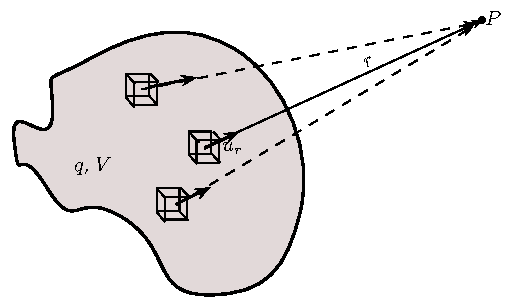
\includegraphics[scale=0.9]{electrostatica/campoelectricocontinuo}
\label{figcontinuo}
\end{center}
\caption{Campo eléctrico generado pora una carga $q$}
\label{campoelectricocontinuo}
\end{figure}

Para el caso general de una distribución de carga volumétrica, superficial o lineal; el campo eléctrico se calcula con la siguiente expresión:

\begin{equation}
\vec{E}(r)=k_e\int_q \dfrac{dq}{r^2}\hat{u}_r,
%\label{ecucampogcontinuo}
\end{equation} 

donde la integral debe hacerse sobre todo el cuerpo de carga $q$ (Figura \ref{campoelectricocontinuo}). Note que que el la ecuación anterior, el vector unitario $\hat{u}_r$ y la magnitud $r$ son variables al igual que $dq$. 

\subsection*{Dipolo eléctrico}

Dos cargas eléctricas opuestas, separadas una distancia $d=2a$, forman lo que llamaremos un dipolo eléctrico (Figura \ref{dipolo}). 

\begin{figure}
\begin{center}
\includegraphics[scale=0.8]{electrostatica/dipolo}
\end{center}
\caption{Dipolo eléctrico}
\label{dipolo}
\end{figure}

El campo eléctrico en un punto $(0,y)$ está dado por:
\begin{eqnarray}
\nonumber
\vec{E}_{y}&=&\vec{E}_{+}+\vec{E}_{-}\\\nonumber
&=& k \dfrac{q}{y^2+a^2}(\cos\theta \hat{i}+\sin\theta \hat{j}) + k \dfrac{q}{y^2+a^2}(\cos\theta \hat{i}-\sin\theta \hat{j})\\
&=& k \dfrac{2qa}{(y^2+a^2)^{3/2}} \hat{i} 
\end{eqnarray}

En general para $y \gg a$, $ \dfrac{1}{(y^2+a^2)^{3/2}} \approx \dfrac{1}{y^3} \approx \dfrac{1}{r^3} $, y así:

\begin{equation}
E _{y}\approx k \dfrac{2qa}{y^3} \hat{i} \approx k \dfrac{2qa}{r^3} = k \dfrac{p}{r^3}
\end{equation}

Donde se define el vector \textbf{momento de dipolo eléctrico $\vec{p}$} como una cantidad vectorial, con módulo $p$ igual al producto de la carga $q$ por la distancia ($d=2a$) que separa las dos cargas, y cuya dirección va de la carga negativa a la carga positiva (Figura \ref{dipolo}). Si una carga de prueba $q_0$ es acercada al dipolo eléctrico, sentirá una fuerza eléctrica, cuya magnitud es: $F=q_0 E \approx k q_0\dfrac{p}{r^3}$.

Ahora, el campo eléctrico en un punto distante sobre el eje $x$, tal que $x \gg a$, es:

\begin{eqnarray}
\vec{E}_x =\vec{E}_{+}+\vec{E}_{-}= \bigg[\dfrac{kq}{(x+a)^2}-\dfrac{kq}{(x-a)^2} \bigg]\hat{i}
\approx -2 \dfrac{2qa}{x^3}\hat{i} \Rightarrow E_x \approx k \dfrac{p}{r^3} ,
\end{eqnarray}
donde $r$ en este caso denota la magnitud del promedio del vector que va de cada una de las cargas al punto de medida del campo eléctrico.

\subsection{Ejemplos de campos eléctricos}

\begin{enumerate}
\item Consideremos un sector circular de un alambre de radio $R$, ángulo $\phi_{0}$ y carga $Q$ uniformemente distribuida. Calculemos el campo eléctrico en el punto $P$ mostrado en la Figura \ref{figsectorcircular}.  

\begin{figure}[h]
\begin{center}
\includegraphics[scale=1.0]{electrostatica/sectorcircular}
\end{center}
\caption{Sector circular}
\label{figsectorcircular}
\end{figure}

\begin{eqnarray}
\vec{E}= k \int_q \dfrac{dq}{r^{2}}\hat{u}_r = k
\end{eqnarray}

\item Un anillo no conductor de radio $R$ está compuesto de dos medios anillos con cargas opuestas $+Q$ y $-Q$, uniformemente distribuidas, tal como se muestra en la figura. Determine el valor del campo y el potencial eléctrico en el punto $P$.

\includegraphics[scale=0.6]{electrostatica/mediosanillos}


\end{enumerate}


\subsection{Movimiento de partículas en presencia de un campo eléctrico}

\begin{figure}
\begin{center}
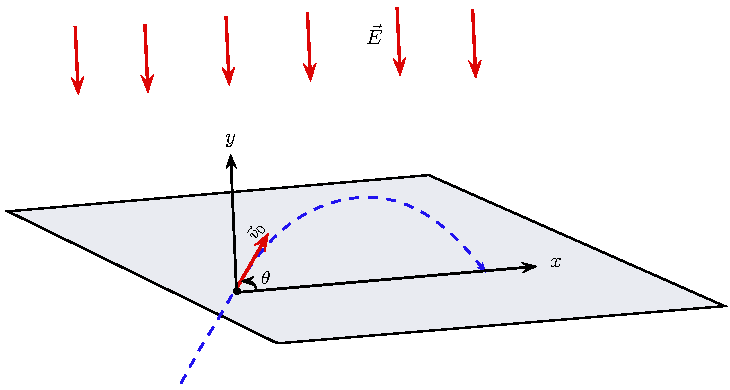
\includegraphics[scale=1.0]{electrostatica/tiroparabolico1}
\end{center}
\caption{Tiro parabólico de una carga $+q$ y masa $m$}
\label{tiroparabolico}
\end{figure}

Supongamos que una partícula positiva de carga $+q$ y masa $m$ ingresa a una región, donde existe un campo eléctrico uniforme y constante, tal como se muestra en la Figura \ref{tiroparabolico}. En este caso, el sistema de coordenadas mostrado en la figura se ha escogido de tal modo que uno de los ejes coordenados tenga la dirección del campo eléctrico. Esto no le quita generalidad al problemas debido a que la escogencia del sistema de referencia no es un absoluto. 

La ecuación de movimiento para la partícula es:

\begin{eqnarray}
\nonumber
\sum_{i} \vec{F}_i &=& m\vec{a} \Rightarrow q \vec{E} + m\vec{g}=m\vec{a} \Rightarrow -qE\hat{j}-mg\hat{j}=-ma_y\hat{j} \\
&\Rightarrow & a_y = \dfrac{qE}{m}+g \approx \dfrac{qE}{m} ,
\end{eqnarray}
donde hemos despreciado los efectos gravitacionales. Esto no siempre es válido, sólo se cumple en ciertos sistemas (ver ejemplo anrerior ... redactar). 
Dado lo anterior, las ecuaciones cinemáticas de posición y rapidez son:

\begin{eqnarray}
x&=&v_0\cos\theta t \\
y&=&v_0\sin\theta t - \dfrac{1}{2}\dfrac{qE}{m}t^2 \\
v_x&=&v_0\cos\theta \\
v_y&=&v_0\sin\theta -\dfrac{qE}{m}t
\end{eqnarray}

Usando las ecuaciones cinemáticas puede mostrarse que el alcance máximo en $x$ y la altura máxima están dados por:

\begin{eqnarray}
x_{max}&=& \dfrac{v_0^2m}{qE}\sin(2\theta) \\
y_{max}&=& ...
\end{eqnarray} 

\begin{figure}[h]
\begin{center}
\includegraphics[scale=0.6]{electrostatica/capacitor1}
\end{center}
\caption{Movimiento cuando la velocidad es perpendicular al campo eléctrico}
\label{figcapacitor1}
\end{figure}

Un caso muy particular sucede cuando la velocidad de la partícula es perpendicular o paralela  al campo eléctrico. Supongamos que una partícula positiva $q_0$ con velocidad $\vec{v}_0$ entra a una región donde existe un campo eléctrico perpendicular a su velocidad, por ejemplo, un campo eléctrico generado por un par de placas paralelas tal como se muestra en la Figura \ref{figcapacitor1}. Las ecuaciones cinemáticas de posición y rapidez para el sistema de referencia mostrado son:

\begin{eqnarray}
x&=&v_0t \\
v_x&=&v_0=cte.\\
y&=&y_0+\dfrac{1}{2} \dfrac{q_0 E}{m}t^2 \\
v_y&=& \dfrac{q_0 E}{m}t 
\end{eqnarray}

\subsection*{EJEMPLO:} Un electrón entra justo por la mitad de un par de placas parelas, las cules están generando un campo eléctrico constante $E=200$ N/C, perpendicular a la velocidad inicial. Su rapidez inicial es $v_0=3.0 \times 10^6$ m/s,  y la longitud horizontal de las placas es $l=0.1$ m.

La magnitud de la aceleración del electrón mientras está en el interior de las placas es:

\begin{eqnarray*}
a=\dfrac{eE}{m}=\dfrac{1.6 \times 10^{-19} \mbox{C} \times 200 \hspace{0.1 cm} \mbox{N/C}}{9.11 \times 10^{-31} \mbox{kg}} \approx 3.51 \times 10^{-13} \mbox{m/s}^2 .
\end{eqnarray*}

La mínima separación $h$ de las placas para que el electrón salga de ellas, se obtiene evaluando las ecuaciones de movimiento para $x=l$ y $y=h/2$.

\begin{eqnarray}
\nonumber
x&=&v_0t=l \Rightarrow t=\dfrac{l}{v_0} \\ \nonumber
y&=&\dfrac{1}{2} a t^2 = \dfrac{1}{2} (3.51 \times 10^{-13} \mbox{m/s}^2) (\dfrac{l}{v_0})^2 = \dfrac{h}{2} \Rightarrow h=3.9 \times 10^{-2} \mbox{m}.
\end{eqnarray}

\subsection*{Ejercicio:}
En el tubo de rayos catódicos un electrón es acelerado horizontalmente desde el reposo por una diferencia de potencial $V_{1}$. Luego ingresa por la mitad de dos placas paralelas conductoras de largo $l$, separadas una distancia $h$ y sometidas a una diferencia de potencial $V_{2}$, tal como se muestra en la figura \ref{figplacas}.
\begin{enumerate}
\item Encuentre el valor de $V_1$ en términos de $l,h$ y $V_2$ para que el electrón salga justo rozando la placa superior, tal como se muestra en la figura.
\item Halle el ángulo $\theta$ en términos de $h$ y $l$, que forma la velocidad del electrón con la horizontal, al salir de las segundas placas.
\end{enumerate}

\begin{figure}[h]
\begin{center}
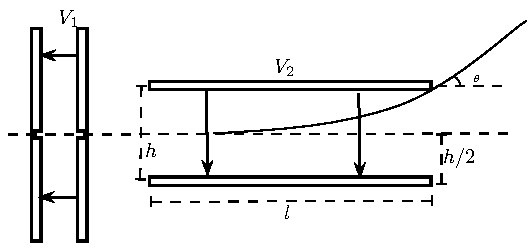
\includegraphics[scale=0.8]{electrostatica/placas}
\end{center}
\caption{Electrón acelerado por un par de placas paralelas}
\label{figplacas}
\end{figure}

\section{Potencial y energía potencial eléctrica}

Es conocido que una fuerza central es conservativa. Dado esto, es posible definir una función energía potencial $E_p(r)=U(r)$ y una función potencial $V(r)$ para dicha fuerza.

\subsection{Diferencia de potencial eléctrica}

\begin{figure}
\begin{center}
\includegraphics[scale=0.6]{electrostatica/diferenciadepotencial}
\end{center}
\caption{Trayectoria seguida por una carga puntual $q_0$ moviendose desde el punto $A$ hasta el punto $B$}
\label{figdiferenciadepotencial}
\end{figure}

Supongamos que una carga puntual $q_0$ se desplaza desde el punto $A$ hasta el punto $B$ debido a su interacción con la carga $Q$ Figura \ref{figdiferenciadepotencial}. El trabajo realizado por la fuerza eléctrica que actua sobre la carga puntual es:

\begin{eqnarray}
dW=\vec{F}\cdot d\vec{l}= q\vec{E}\cdot d\vec{l} \Rightarrow W = q_0 \int_A^B \vec{E}\cdot d\vec{l} ,
\end{eqnarray}

donde $d\vec{l}$ es un diferencial en la dirección de la trayectoria. Además, como el sitema es conservativo, entonces, el trabajo realizado por la fuerza eléctrica debe ser tal que $W=-\Delta U$, es decir, \textit{la variación en la energía potencial del sistema es}:

\begin{eqnarray}
\boxed{\Delta U=-q_0 \int_A^B \vec{E}\cdot d\vec{l} }
\end{eqnarray}

Dado lo anterior, se define la diferencia de potencial $\Delta V$, como la diferencia de energía potencial eléctrica por unidad de carga, es decir:

\begin{eqnarray}
\boxed{\Delta V(r)=V_B-V_A = \dfrac{\Delta U(r)}{q_0} = - \int_A^B \vec{E}\cdot d\vec{l} }
\end{eqnarray}

En general, la diferencia de potencial eléctrica entre los puntos $A$ y $B$ depende del campo eléctrico que asu vez depende de la distribuición de carga $Q$. Diremos que el potencial eléctrico al igual que el campo eléctrico es gerado por la carga $Q$.
La unidad en el sistema internacional SI para la diferencia de potencial será el Volt (V). Diremos que un $1$ V$= 1$ J/C. Otra unidad común en física subatómica es el electronvolt (electronvoltio) $1$ eV$=$ e J $\approx 1.609 \times 10^{-19}$ J.

\subsection{Potencial eléctrico para una partícula puntual $Q=q$}
Si $Q$ es una partícula puntual, entonces, la diferencia de potencial $\Delta V$ entre los puntos $A$ y $B$ es:

\begin{eqnarray}
\Delta V&=&V_B-V_A =-\int_A^B \dfrac{k_eq}{r^2}\hat{u}_r \cdot d\vec{l} =-k_eq\int_A^B \dfrac{\hat{u}_r \cdot d\vec{l}}{r^2} \\ 
&=&-k_eq\int_A^B \dfrac{dr}{r^2}=k_eq \bigg(\dfrac{1}{r_B}-\dfrac{1}{r_A} \bigg),
\end{eqnarray}

donde $r_A$ y $r_B$ son las magnitudes del vector posición que va desde la carga $q$ que genera el campo eléctrico hasta la posición inicial y final de la trayectoria. Note que dicha diferecia de potencial no depende de la trayectoria seguida, solo depende de los puntos inicial y final. Esto es justamente una característica de tener una fuerza y un campo conservativo. Dado lo anterior, definimos el potencial eléctico generado por una partícula puntual $q$ a una distacnia $r$ como:

\begin{eqnarray}
V(r)= k_e \dfrac{q}{r} ,
\end{eqnarray}

donde se toma el cero de potencial eléctrica en el infinito, es decir, $V(\infty)=0$. Dado esto, no hay ambiguedad en hablar de potencial eléctico, refieriendonos a diferencia de potencial eléctrica, ya que $\Delta V = V(r) - V(\infty) \equiv V(r)$.

Es imporante tener en cuenta que para distribuciones de carga $q$, el potencial eléctrico se calcula mediante la integral:

\begin{equation}
\boxed{V(r)= K_e \int_q \dfrac{dq}{r} } , 
\end{equation}
donde el límite de integración inferior es algo simbólico. Quiere decir que la integral debe hacerce barriendo el cuerpo de carga $q$.

\subsection{Relación entre el campo y el potencial eléctico}

Note que la magnitud del campo eléctrico $E(r)$ para una carga puntual $q$ y el potencial eléctrico son tales que:

\begin{eqnarray}
E(r)= k_e \dfrac{q}{r^2}=- \dfrac{\partial }{\partial r }(k_e \dfrac{q}{r} ) \equiv - \dfrac{\partial }{\partial r } V(r), 
\end{eqnarray}

en general, se cumple que:

\begin{eqnarray}
\boxed{\vec{E}(r)= - \vec{\nabla}V(r) } ,
\end{eqnarray}
donde $\vec{\nabla}$ es el operador gradiente en las distintas coordenada en las cuales estemos trabajando. Por ejemplo, en coordenadas cartecianas y en coordenadas esféricas:

\begin{eqnarray}
\vec{\nabla}&=& \hat{i}\dfrac{\partial}{\partial x}+\hat{j}\dfrac{\partial}{\partial y}+\hat{k}\dfrac{\partial}{\partial z} \\ 
\vec{\nabla}&=& \hat{u}_r\dfrac{\partial}{\partial r}+\dfrac{1}{r} \hat{u}_\theta\dfrac{\partial}{\partial \theta}+ \dfrac{1}{r \sin \theta} \hat{u}_{\phi}\dfrac{\partial}{\partial \phi}.
\end{eqnarray}

\subsection{Ejemplo de potencial eléctrico}

\subsection*{Ejemplo:} 
Potencial eléctrico de una esfera maciza aislante de radio $R$ y carga $Q$ uniformemente distribuida (Figura \ref{figpotencial-esfera}).

\begin{figure}
\begin{center}
\includegraphics[scale=0.7]{electrostatica/potencial-esfera}
\end{center}
\caption{Esfera de radio $R$}
\label{figpotencial-esfera}
\end{figure}

\begin{enumerate}

\item Afuera de la esfera ($r \geq R$). Determinemos la diferencia de potencial entre dos puntos externos $A$ y $B$:

\begin{eqnarray}
\nonumber
\Delta V &=& V_A-V_B = - \int_B^A \vec{E} \cdot d\vec{l} = - \int_{r_B}^{r_A} k \dfrac{Q}{r^2}\hat{u}_r \cdot dr\hat{u}_r =-kQ \int_{r_B}^{r_A} \dfrac{dr}{r^2} \\ 
&=& kQ \bigg[ \dfrac{1}{r_A} - \dfrac{1}{r_B} \bigg]   
\end{eqnarray}
En general, para un punto externo a la esfera, cuya distancia al centro sea $r=r_B$, el potencial eléctrico se define como:
\begin{eqnarray}
\boxed{V(r)= k \dfrac{Q}{r}} \hspace{0.5 cm} r \geq  R,
\end{eqnarray}
es decir, es justo el potencial generado por una carga puntual $Q$. Note que $V(\infty)=0$ (es como tomar el punto $A$ a una distacia infinita).

\item Dentro de la esfera ($r \leq R$). Determinemos la diferencia de potencial entre los puntos $C$ y $D$, donde el punto $C$ está justo en la superficie de la esfera y de acuerdo al resultado anterior $V_C= kQ/R$:

\begin{eqnarray}
\nonumber
\Delta V &=& V_C -V_D =  \dfrac{kQ}{R} - V_D \\ \nonumber
&=&-\int_D^C \vec{E}_{\mbox{int}} \cdot d\vec{l} 
= -\int_{r_D}^{r_C} kQ \dfrac{r}{R^3}\hat{u}_r \cdot dr\hat{u}_r \\
&=&-\int_{r_D}^{R} kQ \dfrac{r}{R^3} dr = - \dfrac{kQ}{2R^3} (R^2 - r_D^2),
\end{eqnarray}
así, el potencial eléctrico en el punto $D$ a una distancia $r_D=r$ está dado por:

\begin{eqnarray}
\boxed{V(r)=\dfrac{kQ}{2R} \bigg(3-\dfrac{r^2}{R^2}\bigg)} \hspace{0.5 cm} r \leq  R .
\end{eqnarray}

Note que el potencial es continuo en la superficie de la esfera aislante (Hacer Figura).

\end{enumerate}


\subsection{Potencial eléctrico debido a conductores cargados}

Por definición, un conductor el aquel que permite que las cargas se muevan con facilidad, así, en condiciones de equilibrio electrostático, todas las cargas eléctricas en un conductor sienten fuerzas de repulsión, moviendosen hacia la superficie de dich conductor. En la Figura \ref{figconductor1} se muestra un corte tarnaversal de un cuerpo conductor cargado positivo.  

\begin{figure}
\begin{center}
\includegraphics[scale=0.8]{electrostatica/conductor1}
\end{center}
\caption{Campo eléctrico de un conductor cargado eléctricamente positivo}
\label{figconductor1}
\end{figure}

Las caractrísticas básicas de un conductor son:

\begin{enumerate}
\item La superficie del conductor es una superficie equipotencial, de lo contrario, las partículas sobre la superficie estarían en movimiento y no estariamos en equilibrio electrostático. Esto puede deducirse del hecho de que el campo eléctrico es perpendicular a la superficie, tal como se muestra en la Figura \ref{figconductor1}.
\begin{eqnarray}
\Delta V=V_B-V_A=-\int_A^B \vec{E} \cdot d\vec{l} = 0 \Rightarrow V_A=V_B
\end{eqnarray}
\item El campo eléctrico en el interior del conductor es nulo ya que no hay cargas internas al conductor y ellas son las fuentes de los campos eléctricos. 
\item El potencial eléctrico en el interior del conductor es constante e igual al potencial en la superficie.
\begin{eqnarray}
\Delta V = V_C -V_A = -\int_A^C \vec{E} \cdot d\vec{l} = 0 \Rightarrow V_C=V_A ,
\end{eqnarray}
donde tuvimos en cuenta que el campo eléctrico en el interior es nulo.

\end{enumerate}

En general, en un conductor el campo el?trico y la densidad de cargas superficial son más grandes en las regiones de menor radio de curvatura, es decir, en las regiones más puntudas (\textit{efecto corona}).

\subsection*{Ejemplo:} 
Potencial eléctrico de una esfera maciza conductora de radio $R$ y carga $Q$.

El potencial eléctrico en el exterior de una esfera  carga neta $Q$ está dado por:

\begin{eqnarray}
V(r)= k \dfrac{Q}{r} \hspace*{0.5 cm} r \geq R ,
\end{eqnarray}
note que esto es independiente de que la esfera sea o no sea conductora. Ahora, para $r \leq R$, el potencial tiene el mismo valor, justo el valor que toma el potencial en la suerficie:

\begin{eqnarray}
V(r) = k \dfrac{Q}{R} \hspace*{0.5 cm} r \leq R.
\end{eqnarray}

Note que el potencial es continuo en la superficie de la esfera aislante (Hacer Figura).

\section{Ley de Gauss}

La ley de Gauss nos establece un método alternativo para el cálculo de campos eléctricos de configuraciones de carga altamente simétricas. La ley de Gauss nos establece una relación directa entre los que es el flujo eléctrico que defineremos a continuación y la carga eléctrica que está generando el campo eléctrico.

\subsection*{Flujo eléctrico $\Phi_E$:}

\begin{figure}[h]
\begin{center}
\includegraphics[scale=0.7]{electrostatica/gauss1}
\end{center}
\caption{Flujo eléctrico atravezando la superficie $S$}
\label{figgauss1}
\end{figure}

El flujo eléctrico $\Phi_E$ que atravieza una superficie $S$ se define como:

\begin{eqnarray}
\boxed{\Phi_E=\int_S \vec{E} \cdot d\vec{S} = \int_S E dS \cos \theta } ,
\end{eqnarray}
donde, la integral debe hacerce sobre la superficie $S$ (Figura \ref{figgauss1}). El flujo eléctrico es debido a las líneas de campo que atraviezan la superficie $S$. 
En general el vector $d\vec{S}$ que se define perpendicular a la superficie, no es paralelo al vector de campo eléctrico $\vec{E}$, cuya dirección va determinada por la distribuición de carga $Q$ que lo genera. 

\subsection*{Ejemplo:}

Una carga puntual $q$ está localizada sobre el eje de un anillo de radio $R$ a una distancia $z$ del plano del disco tal como se muestra en la Figura \ref{figflujo1}. Calculemos el flujo eléctrico que atravieza el disco en función de $z$.% e interpretemos el caso particular de $z=R/\sqrt{3}$.

\begin{figure}[h]
\begin{center}
\includegraphics[scale=0.8]{electrostatica/flujo1}
\end{center}
\caption{Flujo a través de un anillo}
\label{figflujo1}
\end{figure}

\begin{eqnarray}
\nonumber
\Phi_E &=& \int_S \vec{E} \cdot d \vec{S} = \int_S k \dfrac{q}{r^2}\hat{u}_r \cdot dS \hat{k} = \int_S k \dfrac{q}{r^2}\cos\theta dS\\
&=&  \int_S k \dfrac{q}{r^2}\dfrac{z}{r} dS = kqz\int_0^R \dfrac{2\pi\rho d\rho}{(\rho^2+z^2)^{3/2}} \\ \nonumber
&=& \dfrac{q}{2 \epsilon_0 }\bigg(1-\dfrac{z}{\sqrt{R^2+z^2} } \bigg)
\end{eqnarray}

\vspace*{0.5 cm}

\begin{figure}[h]
\begin{center}
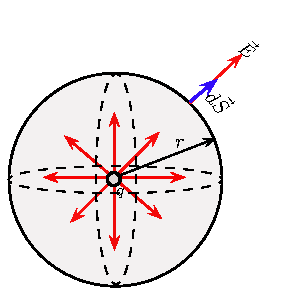
\includegraphics[scale=0.8]{electrostatica/gauss3}
\end{center}
\caption{Gaussiana para una partícula puntual}
\label{figgauss3}
\end{figure}

Para introducir la ley de Gauss, supongamos que una partícula puntual $q$ es encerrada por una superficie esférica ``imaginaria'', concéntrica con la carga. Dicha superficie será llamada, \textit{superficie gaussiana} Figura \ref{figgauss3}. El flujo eléctrico que atravieza dicha superficie:

\begin{eqnarray}
\nonumber
\Phi_E &=& \int_S \vec{E} \cdot d\vec{S} = \int_S E dS = E \int_S dS = E S =E (4\pi r^2) \\
&=& \big(\dfrac{q}{4\pi \epsilon_0 r^2 } \big) (4\pi r^2) = \dfrac{q}{\epsilon_0 } .
\end{eqnarray}

\begin{figure}[h]
\begin{center}
\includegraphics[scale=0.8]{electrostatica/gauss2}
\end{center}
\caption{Ley de Gauss}
\label{figgauss2}
\end{figure}

Aunque el resultado anterior se obtuvo para el caso particular de una carga puntual, es un resultado general conocido  como la \textbf{ley de Gauss}: El flujo neto $\Phi_E$ generado por una carga interna $q_{\mbox{int}}$  y que atravieza una superficie imaginaria $S$, conocido como superficie gaussiana Figura \ref{figgauss2}, es igual $Q_{\mbox{int}}/\epsilon_0$, es decir;

\begin{equation}
\boxed{\Phi_E =  \displaystyle\oint _S \vec{E} \cdot d\vec{S} \equiv \dfrac{Q_{\mbox{int}}}{\epsilon_0 } } 
\end{equation}

\subsection{Ley de Gauss en función del potencial eléctrico}

\subsection{Ejemplos: Ley de Gauss}

...

%%%++++++++++++++++++++++++++++++++++++
%\end{document}


